\section{Design Pattern VS Design Principle}

Un design pattern sbalisce la linea guida su cosa è giusto e su cosa è sbagliato quando si fa il design di un’applicazione, dice cosa fare (e non fare) e non come farlo.

Un design pattern è una soluzione generica e riusabile per un problema comune, dicono come risolvere un problema in un certo contesto software, fornendo chiare linee guida.

\chapter{ACRONIMO SOLID}

I principi SOLID prescrivono come organizzare funzioni e dati in classi e come tali classi dovrebbero essere interconnesse.

Lo scopo di questi principi è la creazione di strutture software che tollerano il cambiamento, sono facili da comprendere/testare e sono riusabili in diversi sistemi software.

\section{Single Responsability Principle (SRP)}

Prevede che una classe deve avere una sola responsabilità, ovvero deve avere una e una sola ragione per essere modificata.

Si dice che la classe deve essere 

\begin{itemize}
  \item \textit{coesiva}, ovvero quanto le cose di un certo gruppo hanno ragione di stare insieme;
  \item \textit{loosely coupling}, ovvero deve dipendere il meno possibile dai metodi di altre classi.
\end{itemize}

Se una classe è responsabile di più cose, la si dovrà cambiare più spesso e cambiare frequentemente una classe porta ad avere ripercussioni su tutte quelle classi che dipendono da lei.

Ciò comporterà, ad ogni modifica, nuova ricompliazione e nuovo test dei metodi.

Prima di aggiungere qualcosa di nuovo a una classe ci si dovrebbe interrogare su quale sia la responsabilità di questa classe, se la risposta comprende funzionalità scorrelate congiunte
con un “e” o un “oppure” allora, probabilmente, si sta violando l’SRP.

\section{Open-Closed Principle (OCP)}

Il principio aperto/chiuso stabilisce che le classi debbano essere aperte alle estensioni e chiuse alle modifiche.

Per modifica si intende il cambiamento del codice di una classe esistente ed estensione significa aggiungere nuove funzionalità.

Tutto ciò sta a significare che dovremmo essere in grado di aggiungere nuove funzionalità senza toccare il codice attuale della classe, questo perché ogni volta che modifichiamo il codice,
rischiamo di dare vita a potenziali bug.

Se nell'SRP si cerca di decomporre la responsabilità, qui si cerca di capire quali parti devono essere concrete (da implementare) e quali devono essere astratte (saranno implementate dai 
consumatori del software).

Negli OOP abbiamo a disposizione il meccanismo dell'ereditarità per creare una classe derivata da una già esistente, il meccanismo dell'override per ridefinire un metodo della classe 
padre e la funzionalità del binding dinamico che permette, dato un oggetto, di chiamare il metodo giusto a runtime.

Questo, però, non è detto che basti a rispettare OCP, specialmente se si estende una classe concreta o se la classe derivata si basa, fortemente, su dettagli implementatitivi della superclasse.
Per esempio, voglio estendere una classe, MySet, per contare gli elementi inseriti

\begin{multicols}{2}
  \begin{lstlisting}
    public class MySet<E> {
      public void add(E o) {
      // add the element to the internal set
      }

      public void addAll(Collection<E> c) {
        for (E e : c) {
          add(e);
        }
      }
    }
  \end{lstlisting}
  \columnbreak
  \begin{lstlisting}
    public class MyCountingSet<E> extends MySet<E> {
      private int count = 0;
      
      @Override
      public void add(E o) {
        super.add(o);
        count++;
      }
    } 
  \end{lstlisting}
\end{multicols}

\newpage
Se io modificassi MySet, ad esempio modifico addAll(), non chiamando più dentro add(), allora la mia classe derivata non sarebbe più corretta, in quanto non avremo più un aumento del contatore.

Quindi, per risolvere questo problema, devo modificare la mia classe, facendo override anche del secondo metodo

\begin{multicols}{2}
  \begin{lstlisting}
    public class MySet<E> {
      public void add(E o) {
      // add the element to the internal set
      }

      public void addAll(Collection<E> c) {
        // add directly all elements
        // WITHOUT relying on add
      }
    }
  \end{lstlisting}
  \columnbreak
  \begin{lstlisting}
    public class MyCountingSet<E> extends MySet<E> {
      private int count = 0;
      
      @Override
      public void add(E o) {
        super.add(o);
        count++;
      }

      @Override
      public void addAll(Collection<E> c) {
        super.addAll(c);
        count += c.size();
      }
    } 
  \end{lstlisting}
\end{multicols}

Inoltre, se ad un certo punto tornassi alla versione originale di MySet, avrei lo stesso problema, ovvero MyCountingSet non funzionerebbe più in quanto il contatore verrebbe incrementato due 
volte ogni volta.

Quindi possiamo vedere che le modifiche fatte a MySet possono anche essere giuste o minimali ma sono devastanti per la mia sottoclasse.

Questo porta al concetto della \textbf{fragile base class problem}, ovvero una classe è considerata fragile se piccole modifiche corrette e sicure alla classe base, possono portare le classi 
derivate a non funzionare più correttamente.

Quindi sarebbe meglio proibire l'estensione della classe (con un final), proibire la ridefinizione di alcuni metodi (anche qui final) e documentare come una classe base dovrebbe essere usata/estesa.

Allora, dal concetto di classi concrete ed ereditarietà, arriviamo al concetto di classi astratte o interfacce ed, eventualmente, al principio di composizione e delega.

\begin{wrapfigure}{r}{3cm}
  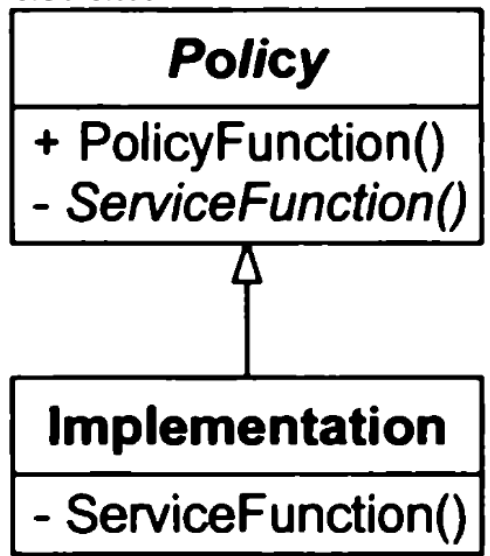
\includegraphics[width=0.5\linewidth]{../../immagini/principio_SOLID/esempioOCP}  
\end{wrapfigure}

Prediamo come esempio la classe astratta Policy che ha un metodo, public e probabilmente final, PolicyFunction che, a sua volta, implementa una certa politica in termini di un metodo, protetto e 
astratto, ServiceFunction.

Policy, quindi, ha una parte concreta (PolicyFunction) ed una astratta (ServiceFunction), si dice che è aperta all'estensione, tramite la parte astratta e chiuse alle modifiche dovute al fatto 
che PolicyFunction è final.

Supponiamo di avere una classe Client che si occupa di fare logging e di voler aggiungere un nuovo tipo di log, basterà, quindi, aggiungere un nuovo tipo di logging ad enum ed un nuovo ramo allo if-else.

Come si vede, la classe è si configurabile rispetto al log ma non è aperta ad estensioni del log in quanto la sua gestione dipende da un if-else/switch e quanfo si usa un if-else/switch, si sta violando 
OCP, inoltre c'è il dubbio su cosa faccia l'ultimo else (in questo caso non fa nulla).

\begin{lstlisting}[linewidth=10cm]
public class Client {
  public enum LogConf { CONSOLE, FILE }
  private LogConf logConf;
  
  public Client(LogConf logConf) { this.logConf = logConf; }
  
  public void aMethod() {
    // do something before or after the log method...
    log("a message");
  }

  private void log(String message) {
    if (logConf == LogConf.CONSOLE) {
    // log to System.out
    } else if (logConf == LogConf.FILE) {
    // log to a File
    } else {
    // what to do?!?
    }
  }
}
\end{lstlisting}

\newpage
Quindi, per risolvere ciò
\begin{itemize}
  \item decidiamo di astrarre la funzionalità di logging attraverso l'interafccia Log che avrà diverse implementazioni come ConsoleLog o FileLog;
  \item la classe Client dichiara una variabile privata di tipo Log;
  \item l’istanza Log viene passata al costruttore;
  \item Client delega completamente il logging all’istanza di Log.
\end{itemize}

La nuova classe è estendibile a nuovi sistemi di logging, infatti basta creare una nuova implementazione di Log, il Client non è stato minimamente toccato, non c'è stato bisogno di ricompilare.

\begin{multicols}{2}
  \begin{lstlisting}
    public class Client {
      private Log logger;
        
      public Client(Log log) {
        this.logger = log;
      }
        
      public void aMethod() {
        // do something...
        log("a message");
        // do something...
      }
    
      private void log(String message) {
        logger.log(message);
      }
    }
  \end{lstlisting}
  \columnbreak
  \begin{lstlisting}
    public interface Log {
      public void log(String message)
    }

    public class ConsoleLog implements Log {...}

    public class FileLog implements Log {...}
  \end{lstlisting}  
\end{multicols}
Ovviamente le due classi concrete fanno override del metodo log.\\
Esempio pratico sono i software basati sui plug-in, ovveri software che non è possibile modificare ma estendibili tramite plug-in.\\

\section{Liskow Substitution Principle (LSP)}
 
Questo principio si basa sul concetto di sottotipo.

In java, un oggetto di tipo T sottotitpo di S, detto supertipo, può essere sempre
\begin{itemize}
  \item assegnato a una variabile dichiarata di tipo S;
  \item passato come argomento di un metodo che si aspetta un parametro di tipo S;
  \item restituito in un metodo il cui tipo di ritorno è S.
\end{itemize}

Per un sottotitpo valgono la proprietà riflessiva, ovvero data una classe A, A è sottotipo di se stessa (si indica con $A<:A$) e la proprietà transitiva, ovvero siano 
A, B e C tre classi, se $A<:B$ e $B<:C\Rightarrow A<:C$.

Il prinicipio di Liskow è qualcosa di più forte della definizione di sottotipo, ovvero, vuole che il comportamento del programma, quando sostituisco S con T, non 
cambia, non si rompe, continua a funzionare correttamente (non significa che non cambia nulla, altrimenti non avrebbe senso).

Per esempio, ho una classe Rectangle con due campi, height e weight, metodi setter ed un metodo area.
\begin{multicols}{2}
  \begin{lstlisting}
  public class Rectangle {
    private int height, width;
    
    public void setHeight(int height) {...}

    public void setWidth(int width) {...}

    public int area() { return height * width;}
  }
  \end{lstlisting}
  \columnbreak
  \begin{lstlisting}
    @Test
    public void testRectangle() {
      Rectangle r = new Rectangle();
      r.setHeight(5);
      r.setWidth(3);
      assertEquals(15, r.area());
    }
  \end{lstlisting}
\end{multicols}

Ora voglio creare la classe Square da rettangolo, tanto basta porre entrambi i lati uguali.\\
\begin{multicols}{2}
  \begin{lstlisting}
    public class Square extends Rectangle {
      
    @Override
      public void setHeight(int height) {
        super.setHeight(height);
        super.setWidth(height);
      }

      @Override
      public void setWidth(int width) {
        super.setWidth(width);
        super.setHeight(width);
      }
    }
  \end{lstlisting}
  \columnbreak
  \begin{lstlisting}
    @Test
    public void testSquare() {
      Square s = new Square();
      s.setHeight(5);
      assertEquals(25, s.area());
      s.setWidth(3);
      assertEquals(9, s.area());
    }
  \end{lstlisting}
\end{multicols}  

Presi singolarmente, i test passano, ora, però, bisogna vedere che, se applicando il principio di sostituzione, tutto rimane invariato.\\
\begin{lstlisting}[linewidth=8cm]
  @Test
  public void testSquareAsRectangle() {
    Rectangle r = new Square();
    r.setHeight(5);
    r.setWidth(3);
    assertEquals(15, r.area());
  }
\end{lstlisting}

Questo test fallisce perchè, quando chiamo in sequenza i due metodi setter, questi saranno chiamati da quadrato e non da rettangolo (binding dinamico).

Quindi Square non è sostituibile a Rectangle anche perchè alla classe Square, alla fine dei conti serve un solo campo.

Per risolvere il problema possiamo pensare di eliminare i due metodi setter ed introdurre un'interafccia, Shape, con all'interno la definizione del metodo area.

Così facendo, entrambe le classi concrete, implementeranno Shape e ridefineranno, a modo loro, il metodo area attraverso override.

\begin{center}
  \begin{tabular}{c}
    \begin{lstlisting}[linewidth=5cm]
      public interface Shape {
        public int area();
      }
  \end{lstlisting}
  \end{tabular}
\end{center}

\begin{multicols}{2}
  \begin{lstlisting}
    public class Rectangle implements Shape {
      private int height, width;
      
      public Rectangle(int height, int width) {
        this.height = height;
        this.width = width;
      }

      @Override
      public int area() { return height * width;}
    }
  \end{lstlisting}
  \columnbreak
  \begin{lstlisting}
    public class Square implements Shape {
      private int side;
      
      public Square(int side) {
        this.side = side;
      }
      
      @Override
      public int area() { return side * side;}
    }
  \end{lstlisting}
\end{multicols}

I test che useranno Shap, passandogli prima Rectangle e poi Square, funzioneranno
\begin{lstlisting}[linewidth=6cm]
  @Test
  public void testShape() {
    Shape s = new Rectangle(5,3);
    assertEquals(15, s.area());
    s = new Square(5);
    assertEquals(25, s.area());
  }  
\end{lstlisting}

Detto in parole povere, bisogna cercare di lavorare, il più possibile, con classi astratte o interfacce, lavorare verso l'astrazione e non verso l'implementazione.

\newpage
\section{Iterafce Segregation Principle (ISP)}

È simile all’SRP ma incentrato su interfacce e client.

Supponiamo di avere a disposizione un'interfaccia contente metodi che svolgono differenti compiti.

Un client che implementerà questa interfaccia, sarà costretto ad implementare tutti i suoi metodi, anche quelli che non gli servono.

Se un client richiedesse una modifica all’interfaccia, anche gli altri client ne sarebbero influenzati, anche se la modifica dovesse riguardare un metodo che a loro
non serve.

Quindi sarebbe conveniente dividere l'interfaccia originale in interfacce più piccole, così facendo l'interfaccia originale conterrà solo i metodi comuni ai client, 
mentre le interfacce più piccole si occuperanno dei metodi specifici.

Prendiamo ad esempio il sistema di pagamento di un parcheggio

\begin{lstlisting}[linewidth=15cm]
  public interface Parcheggio {

    void parcheggiaAuto();	// Diminuisce parcheggi vuoti di 1
    void esceAuto(); // Aumenta parcheggi vuoti di 1
    void getCapienza();	// Restituisce capienza auto
    double calcolaQuota(Auto auto); // Restituisce il prezzo in base al numero di ore
    void faiPagamento(Auto auto);
  }

  class Auto {
    ...
  }
\end{lstlisting}

Immaginiamo di voler implementare un parcheggio gratuito (che estenderà Parcheggio) e notiamo che abbiamo obbligato questa classe ad implementare i metodi di pagamento
del parcheggio anche se non ne avrebbe bisogno (è gratis) e magari, nel metodo pagamento, lanciamo un'eccezione gestita con un semplice "il parchegio è gratis".

Quindi si nota che l'interfaccia Parcheggio si occupa di due logiche distinte, quella del parcheggio e quella del pagamento del parcheggio stesso.

Una possibile soluzione, quindi, sarebbe quella di scindere l'interfaccia parcheggio in altre due interfacce, quella a pagamento e quella gratis, la prima oltre 
ad ereditare i metodi riferiti al parcheggio, aggiungerà i metodi riguardanti i pagamenti, mentre la seconda, implementrà l'interfaccia padre.

Con questo nuovo modello, possiamo anche andare oltre e dividere l'interfaccia pagamento per supportare diverse modalità di pagamento.

\begin{figure}[H]
  \centering
  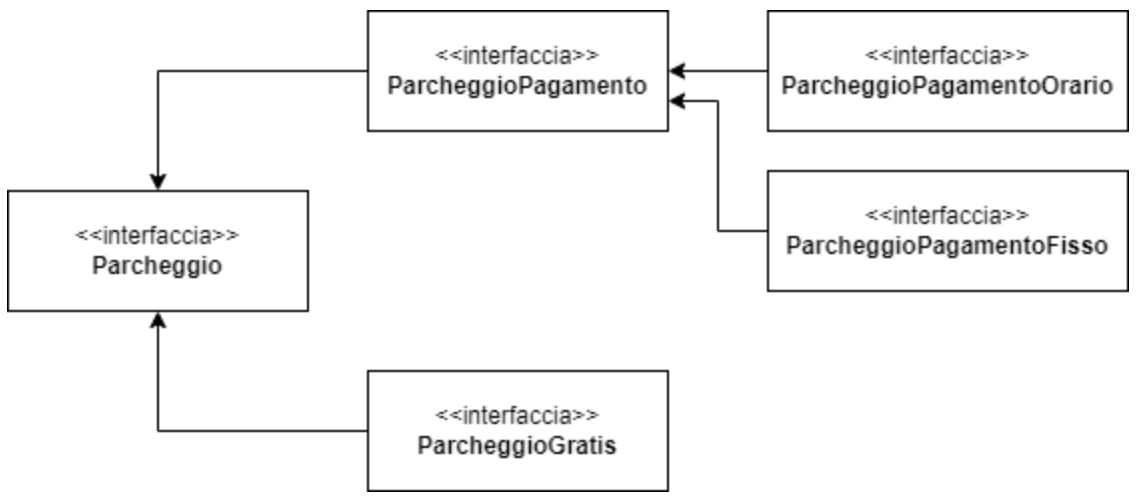
\includegraphics[width=0.5\linewidth]{../../immagini/principio_SOLID/refactoring_interfaccia.png}
\end{figure}

\section{Dependency Inversion Principle (DIP)}

Questo principio ci dice che i sistemi più flessibili sono quelli dove le dipendenze del codice sorgente si riferiscono solo alle astrazioni.

Per dipendenza nel codice sorgente si intende che, dato un file Client.java, se in dato file nomino un tipo A, allora diremo che il codice sorgente di Client dipende 
da A.

Anche se in un dato Client.java useremo un sottotipo di A, B, diremo che Client dipende, staticamente, da A.

Da qui utilizzeremo il concetto di modulo/componente inteso come raggruppamento di classi.

Tradizionalemente, i moduli di alto livello dipendono dai moduli di basso livello, per dipendere si intende chiamare direttamente codice di basso livello o istanziare
direttamente classi concrete.

Per codice di alto livello, detto anche core, intendiamo la parte di un'applicazione computazionale, algoritmica o che elabora, ovvero è la parte che contraddistingue 
un'applicazione.

Mentre per codice di basso livello intendiamo interfaccia utente o database.

Quindi se il codice di alto livello dipende dal codice di basso livello, significa che modifiche a quest'ulitmo, avranno un impatto sul codice di alto livello.

\newpage
Si prende come esempio un'architettura OO dove la parte più alta indica codice di alto livello.
\begin{wrapfigure}{r}{8cm}
  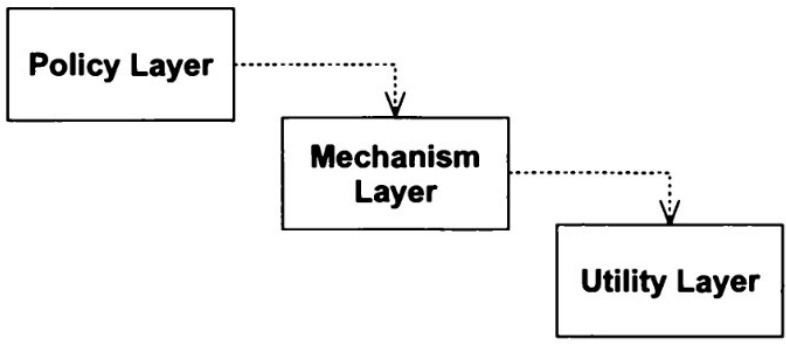
\includegraphics[width=0.5\linewidth]{../../immagini/principio_SOLID/architetturaOOnoDIP}  
\end{wrapfigure}

Il layer di alto livello usa solo il layer sottostante ma usare significa che dipende dal layer sottostante.

Inolte se il layer sottostante dipende dal layer di basso livello, allora il layer di alto livello, transitivamente, dipende dal layer di basso livello.

Per risolvere questo problema
\begin{itemize}
  \item ogni layer di alto livello dovrebbe dichiarare una propria interfaccia per i servizi di cui ha bisogno e farla implementare al layer sottostante;
  \item il layer sottostante implementerà l'interfaccia dichiarata dal layer superiore.
\end{itemize}

Così facendo, le dipendenze vengono invertite, ovvero sono i layer di basso livello a dipendere dai layer di alto livello.
\begin{figure}[H]
  \centering
  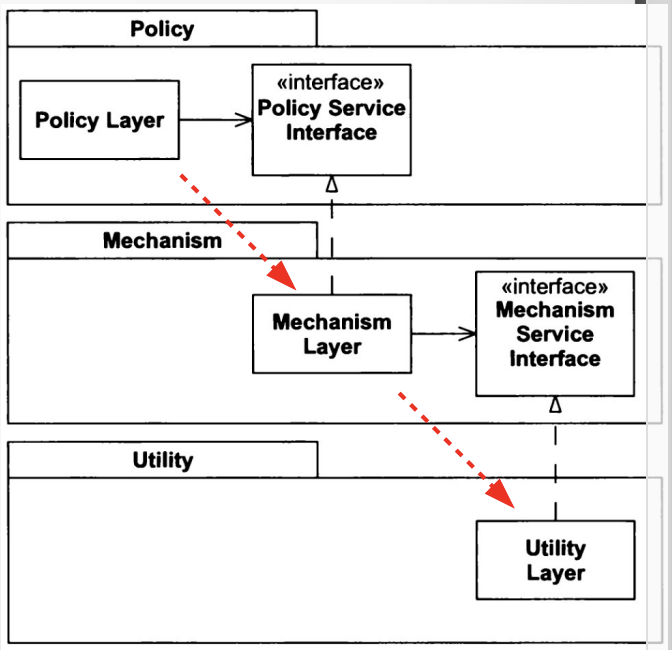
\includegraphics[width=0.35\linewidth]{../../immagini/principio_SOLID/architetturaOODIP}  
\end{figure}

staticamente Policy chiama un metodo dell'interfaccia, a runtime verrà invocato l'implementazione di tale metodo dal layer inferiore, così facendo, posso cambiare un
layer sottostante senza modificare un layer soprastante e posso testare un layer soprastante senza avere un layer sottostante ed inoltre è buona cosa non menzionare 
mai il nome di qualcosa che è concreto (non astratto) e volatile (che cambia spesso) e non avervi riferimento.

Quindi, i design pattern guidano lo sviluppo del codice e il refactoring aiutando a sviluppare software pulito e facile da estendere, riusare, mantenere e testare.